\graphicspath{{./figures}}

% Project Planning
\chapter{Project Planning}
\textcolor{red}{Still to be formulated into a gantt chart}
Week 01 (24/07 to 30/07): Problem formulation; requirements gathering
Week 02 (31/07 to 06/08): Initial research; component selection
Week 03 (07/08 to 13/08): System-level design; initial system layout; components ordered
Week 04 (14/08 to 20/08): PCB design without traces; initial circuit design
Week 05 (21/08 to 27/08): Component prototyping; Full PCB design; initial antenna design;
Week 06 (28/08 to 03/09): Mechanical design; Custom protocol investigation; PCB ordered
Week 07 (04/09 to 10/09): (Test week)
Week 08 (11/09 to 17/09): Initial build
Week 09 (18/09 to 24/09): Software design; initial testing
Week 10 (25/09 to 01/10): Software design; debugging
Week 11 (02/10 to 08/10): Reporting
Week 12 (09/10 to 15/10): Design improvement
Week 13 (16/10 to 22/10): Testing
Week 14 (23/10 to 29/10): Reporting
Week 15 (30/10 to 05/11):

% Schematics
\includepdf[scale=0.65,pages=1,offset=0mm -35mm,pagecommand=\chapter{Schematics}\section{Ground Station}\label{sec:appendix_gs_schematics}]{docs/gs_schematic}
\includepdf[scale=0.7,pages=1,pagecommand=\section{PocketQube Unit}\label{sec:appendix_pq_schematic}]{docs/pq_schematic}
\section{Errata}\label{sec:appendix_pcb_errata}
\begin{itemize}
    \item \textcolor{red}{Full errata for PCB designs still to be added}
\end{itemize}

% Standards
\includepdf[scale=0.8,pages=1,offset=0mm -35mm,pagecommand=\chapter{Standards}\section{PQSU}\label{sec:appendix_pqsu}]{docs/pqsu}
\includepdf[scale=0.85,pages=1,pagecommand=\section{SUNCQ}\label{sec:appendix_suncq}]{docs/suncq}
\includepdf[scale=0.85,pages=2]{docs/suncq}

% Implementations
\chapter{Implementations}
\section{Ground Station}\label{sec:appendix_gs_antenna_original}
\begin{figure}[!htb]
  \centering
  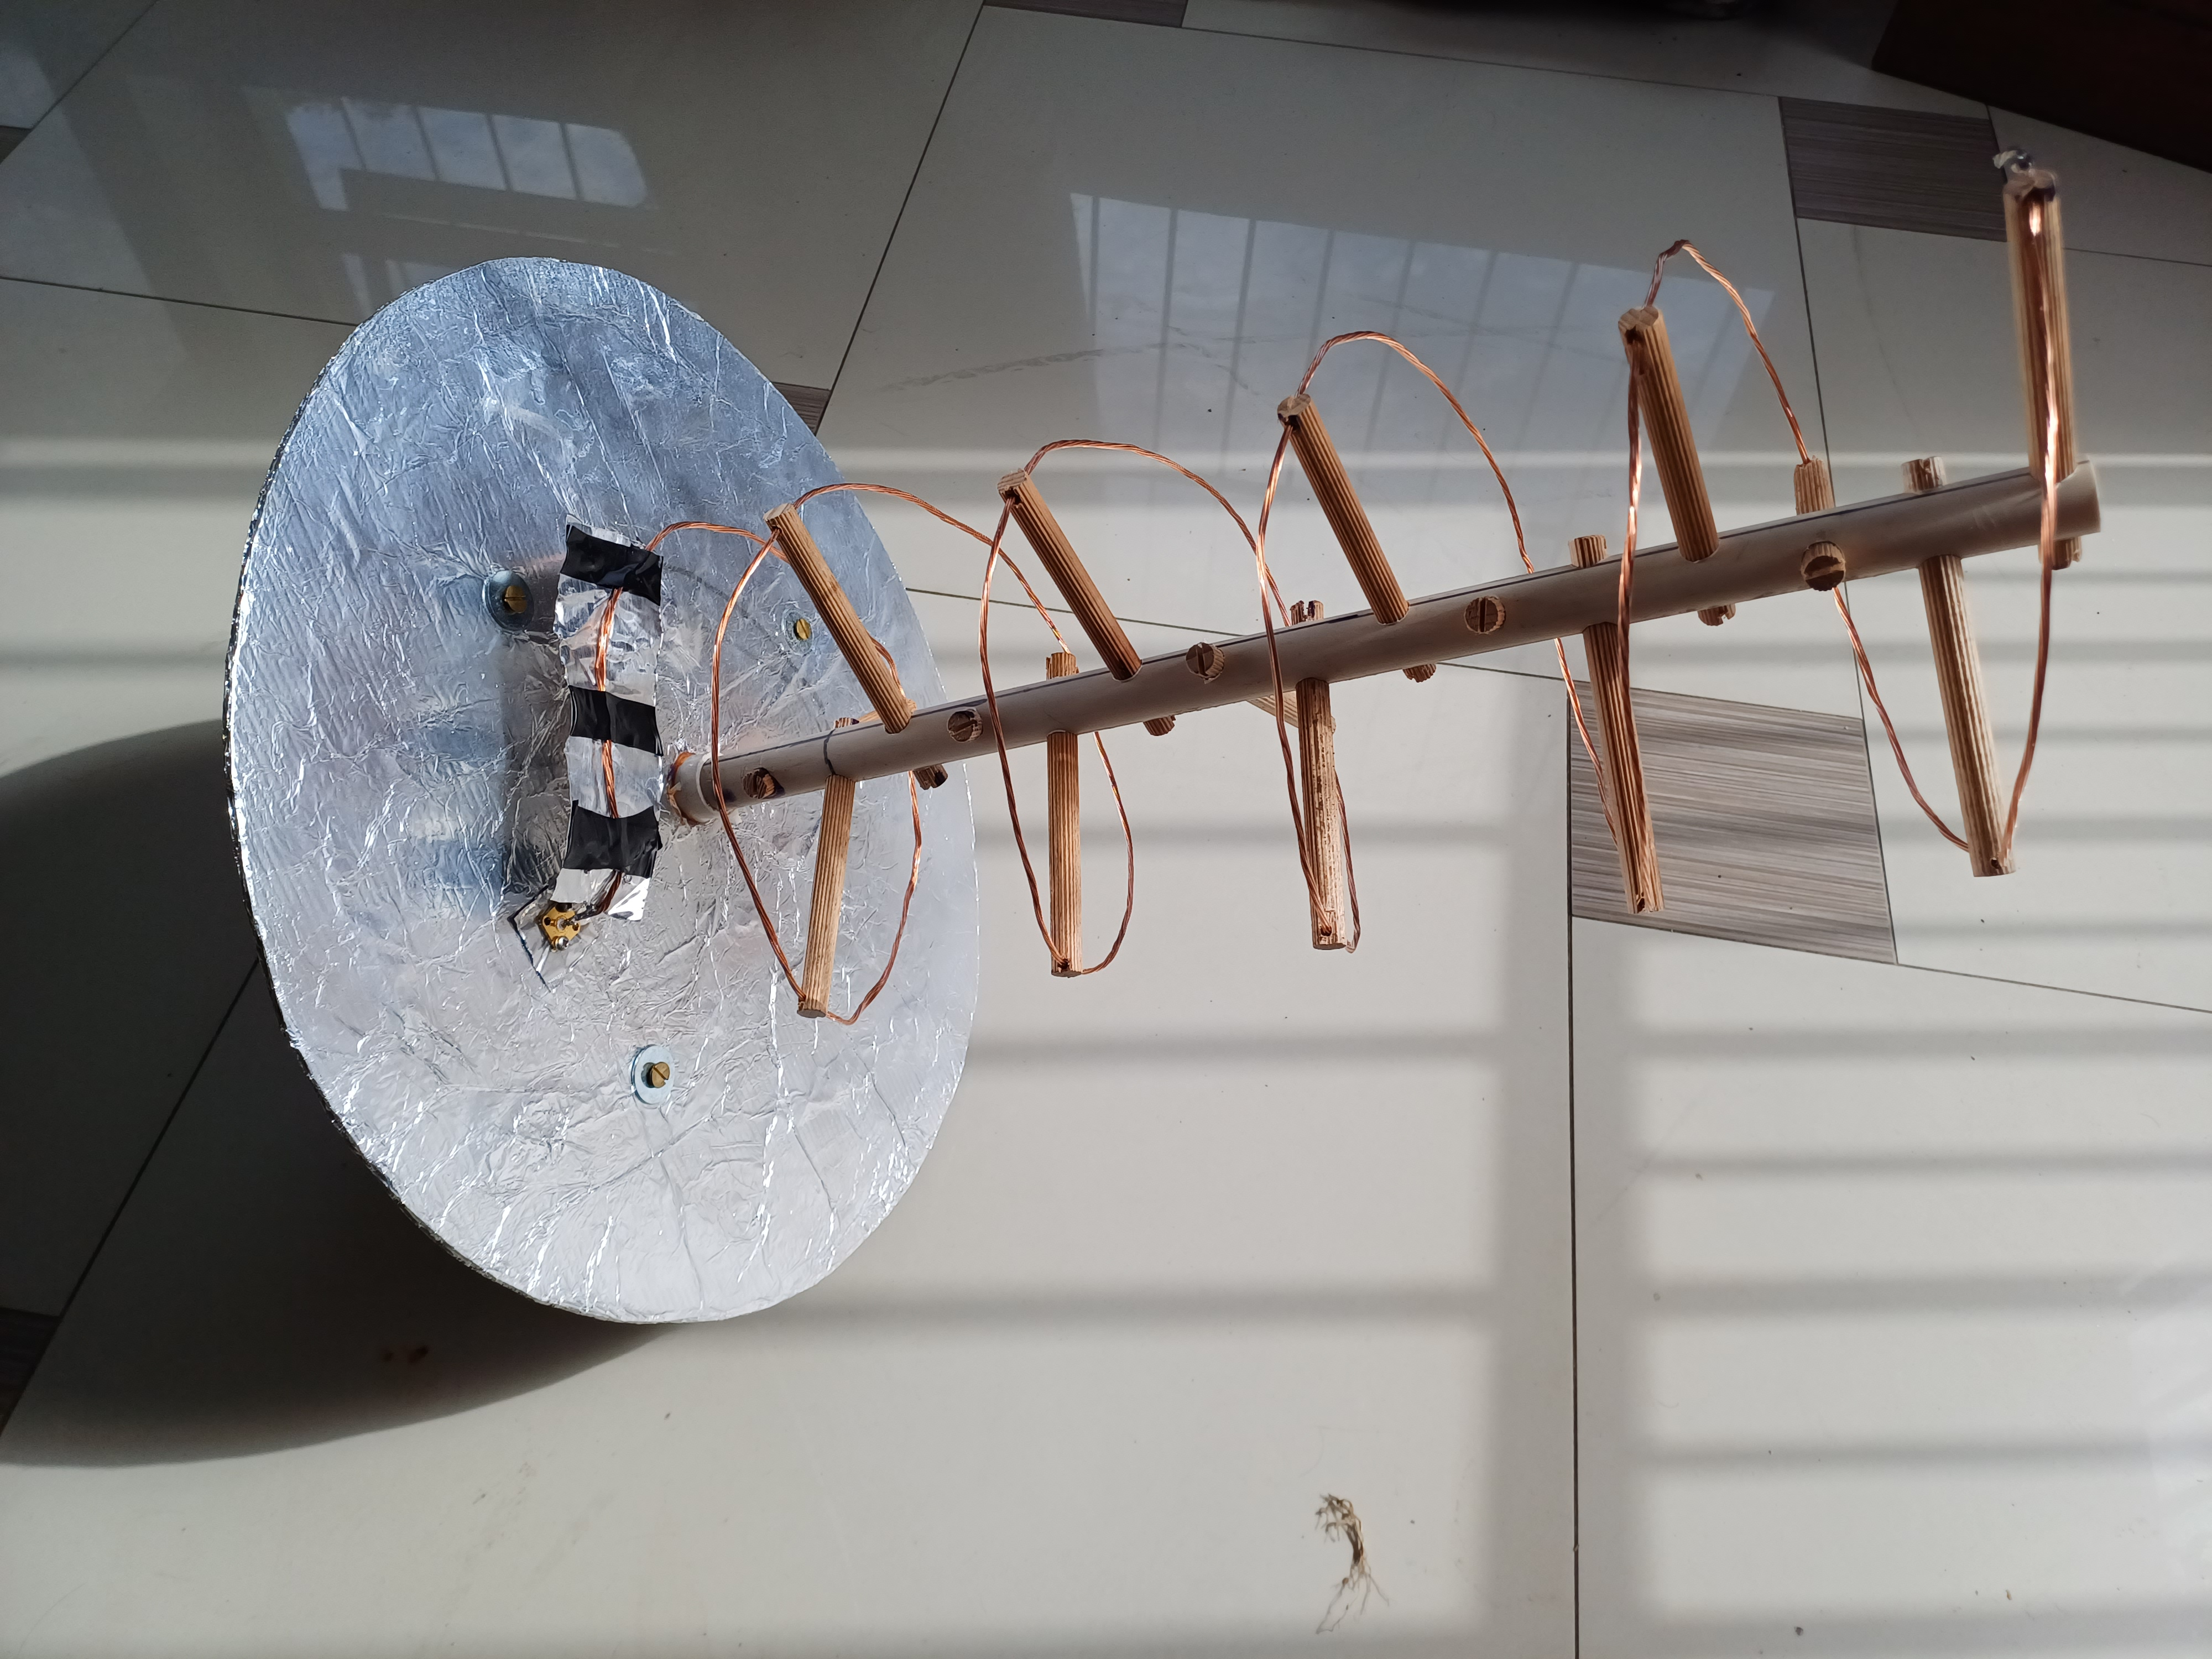
\includegraphics[width=0.9\textwidth]{gsAntennaOriginal}
  \caption{Ground Station Original Antenna Build}
  \label{fig:gsAntennaOriginal}
\end{figure}
\newpage
\section{PocketQube}\label{sec:appendix_pq}
\begin{figure}[!htb]
    \centering
    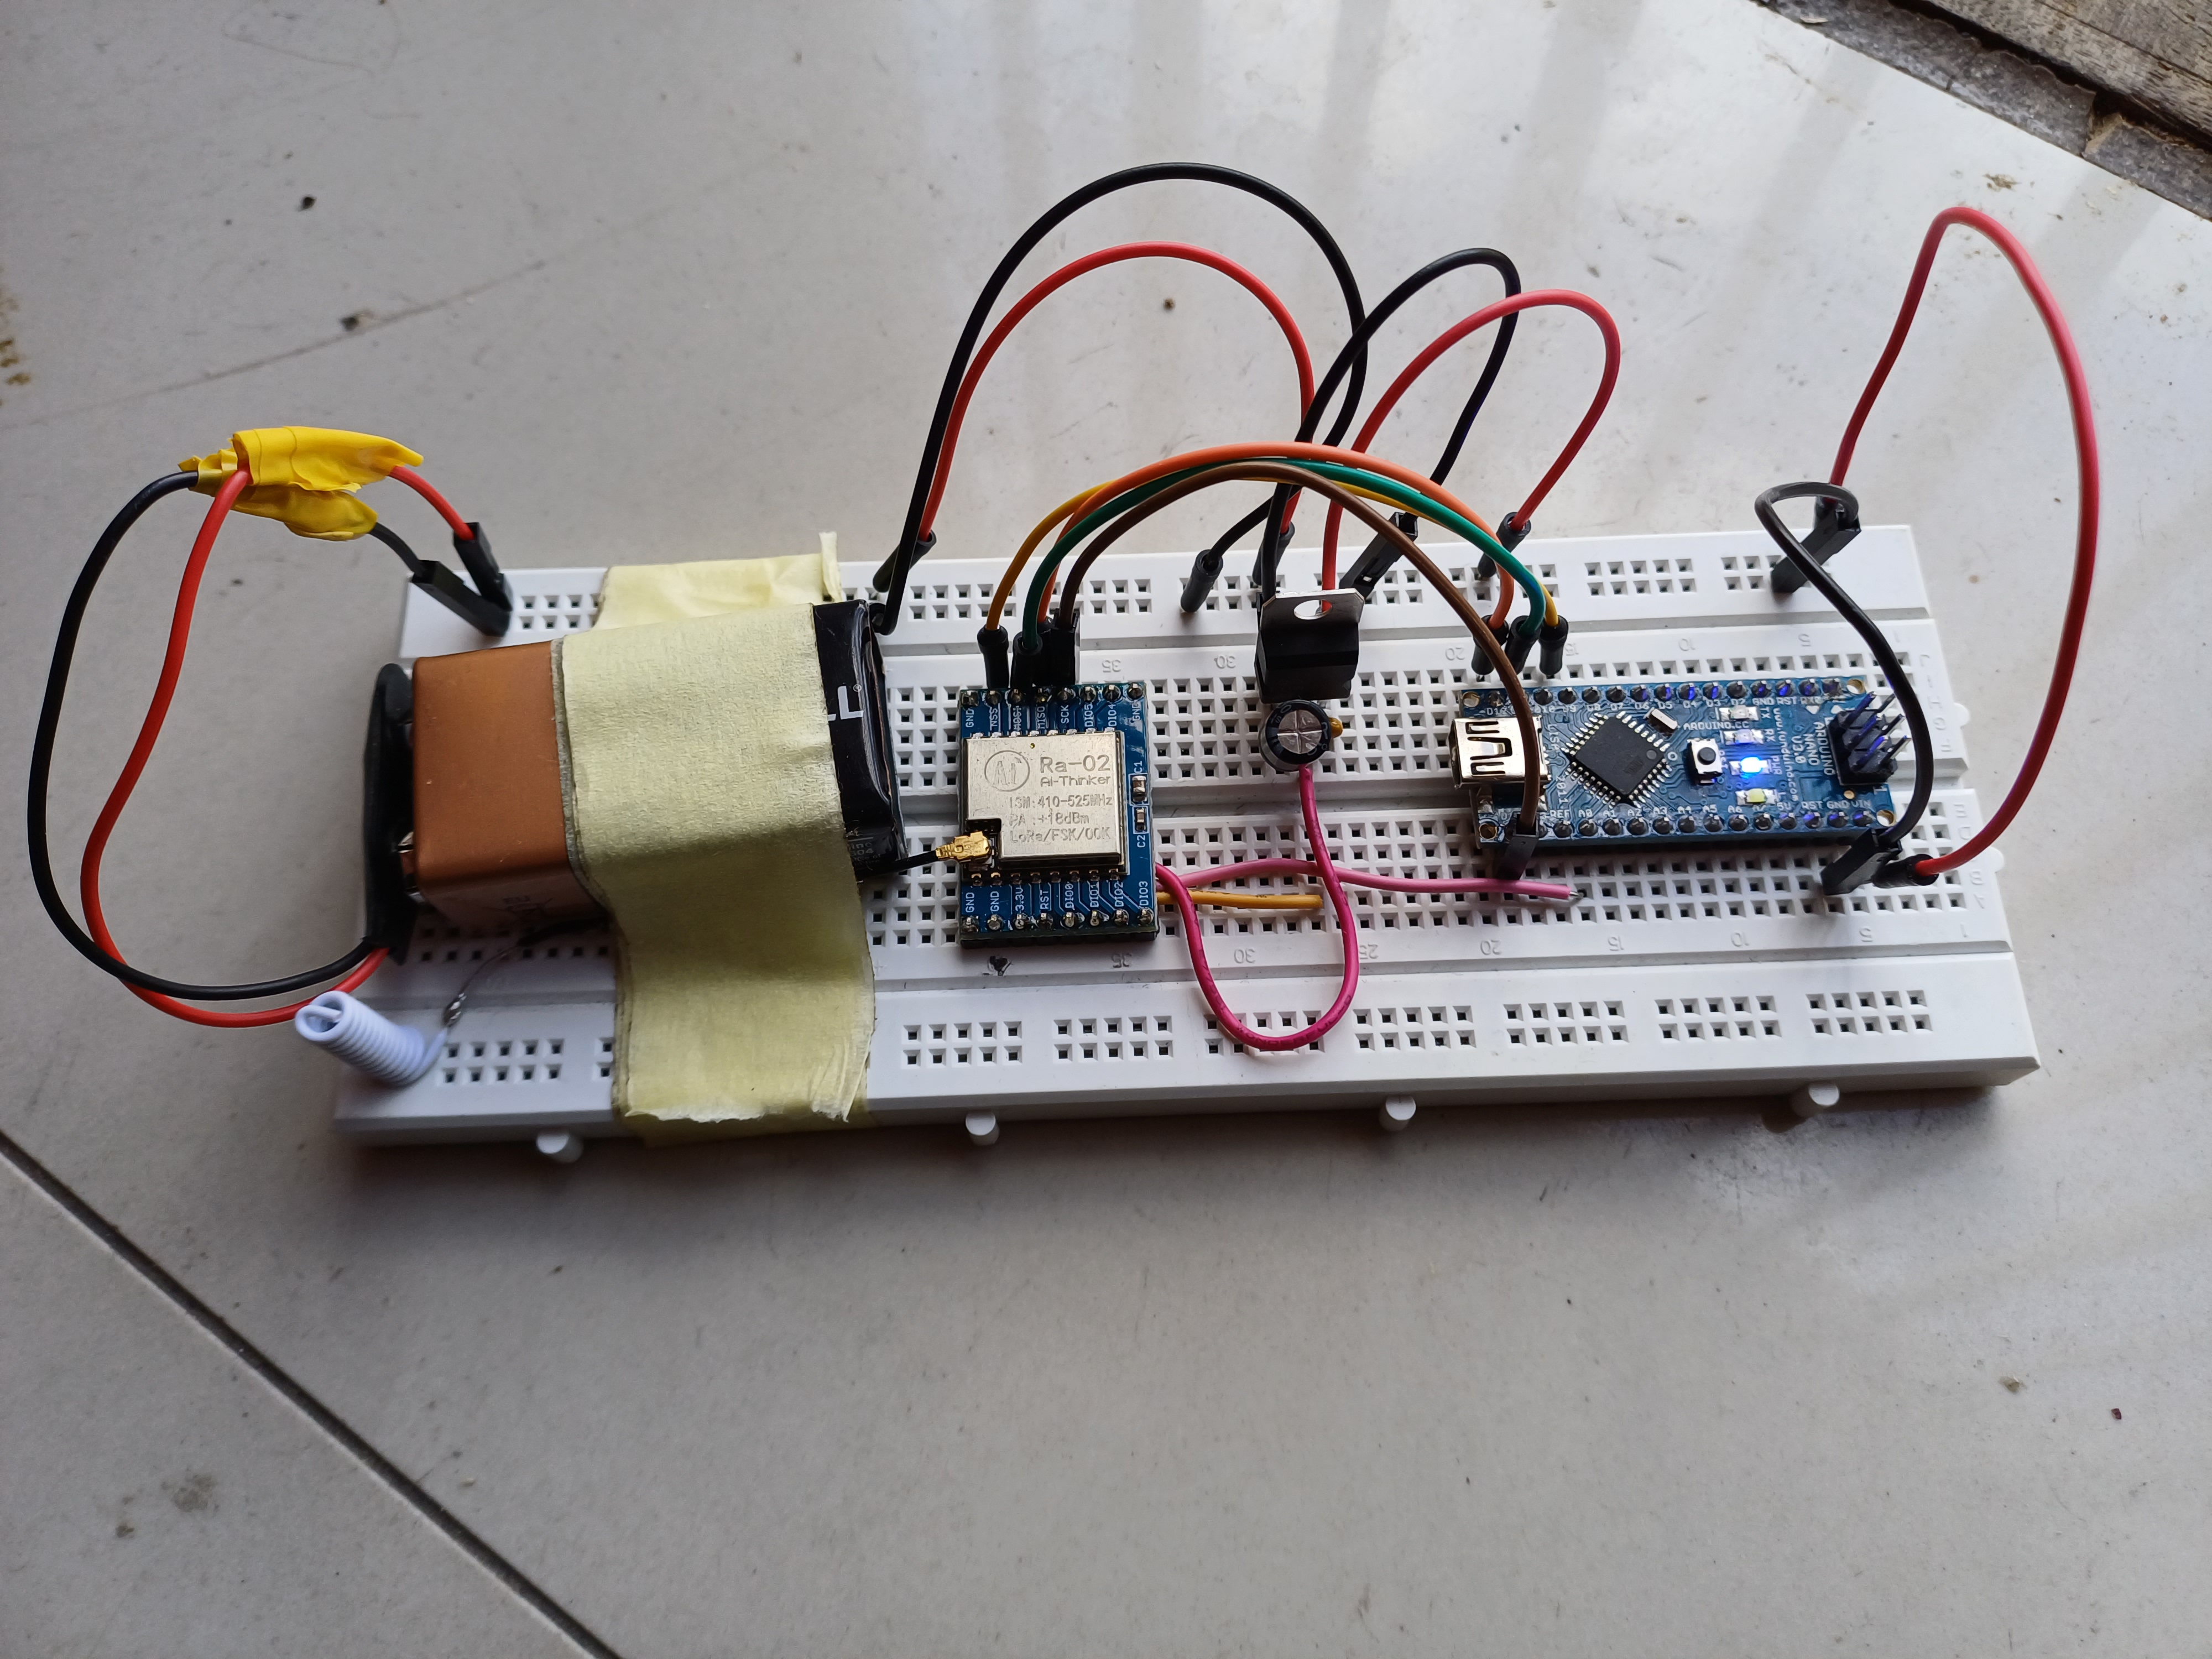
\includegraphics[width=0.8\textwidth]{pqBreadboard}
    \caption{PocketQube Breadboard for Testing}
    \label{fig:pqBreadboard}
\end{figure}
\begin{figure}[!htb]
  \centering
  \includegraphics[width=0.5\textwidth]{pqAntenna}
  \caption{PocketQube Dipole Antenna}
  \label{fig:pqAntenna}
\end{figure}
\newpage
\section{GUI}\label{sec:appendix_gui}
\begin{figure}[!htb]
  \centering
  \includegraphics[width=0.95\textwidth]{guiSnapshot1}
  \caption{GUI Snapshot}
  \label{fig:guiSnapshot}
\end{figure}

% Tests
\chapter{Tests}
\section{Range Tests}\label{sec:appendix_range}
\begin{figure}[!htb]
  \centering
  \includegraphics[width=0.8\textwidth]{rangeTests}
  \caption{Range Test Locations}
  \label{fig:rangeTests}
\end{figure}